%!TEX program = xelatex
%!TEX root = slides.tex
\documentclass[10pt]{beamer}

% XeLaTeX
\usepackage[no-math]{fontspec}
\usepackage[main = russian, english]{babel}
\usepackage{xltxtra}
\usepackage{xunicode}

% Fonts
\setmainfont[
 BoldFont={Open Sans Bold}, 
 ItalicFont={Open Sans Italic},
 BoldItalicFont={Open Sans Bold Italic}
]{Open Sans}
\setsansfont{Open Sans}
\setmonofont{Liberation Mono}

\newfontfamily\ExtraLight{Open Sans Light}
\newfontfamily\Light{Open Sans}
\newfontfamily\Book{Open Sans}
\newfontfamily\BookBold{Open Sans Bold}

\defaultfontfeatures{Scale=MatchLowercase,Mapping=tex-text}

% LENGTHS
\setlength{\parskip}{4pt plus 1pt minus 1pt}
\linespread{1.15}

% Packages
\usepackage{graphicx}
%\usepackage{ifpdf,mla}
\usepackage{hyperref}
\usepackage{tikz}
\usepackage{xcolor}
\usepackage{ifxetex, ifluatex}
\usepackage{listings}
% \usepackage{enumitem}
\usepackage[normalem]{ulem}
\usepackage[font=bf,skip=\baselineskip]{caption}
\hypersetup{colorlinks=true}

\definecolor{dkgreen}{rgb}{0,0.6,0}
\definecolor{mauve}{rgb}{0.5,0.37,0.37}

\lstset{
  frame=lrtb,
  language=c,
  aboveskip=2mm,
  belowskip=2mm,
  showstringspaces=false,
  columns=fullflexible,
  basicstyle={\scriptsize\ttfamily},
  % numbers=left,
  numbers=none,
  numberstyle=\tiny\color{gray},
  keywordstyle=\color{blue},
  commentstyle=\color{dkgreen},
  stringstyle=\color{mauve},
  breaklines=true,
  breakatwhitespace=true,
  tabsize=4,
  backgroundcolor=\color{gray!7},
  showspaces=false,
  showtabs=false,
  escapeinside={(*@}{@*)},
  rulecolor=\color{gray!10}
}
\captionsetup[lstlisting]{font={scriptsize,tt}}

% === Colors ===
\definecolor{cTitle}{HTML}{FF853A}
\definecolor{cFrameTitle}{HTML}{F2F2F2}
\definecolor{cTitleBack}{HTML}{23373B}
\definecolor{cBackground}{HTML}{23373B}
\definecolor{cSeparator}{HTML}{FF473B}
\definecolor{cText}{HTML}{23373B}
\definecolor{cFrameBackground}{HTML}{F2F2F2}
\definecolor{cItem}{HTML}{414141}

\definecolor{cGreen}{HTML}{007A29}
\definecolor{cRed}{HTML}{CC3300}

% setting spectial colors
\setbeamercolor{frametitle}{fg=cFrameTitle, bg=cTitleBack}
\setbeamercolor{title}{fg=cTitle}
\setbeamercolor{progress bar}{fg=cSeparator}
\setbeamercolor{title separator}{fg=cSeparator}
\setbeamercolor{section title}{fg=cTitle}
\setbeamercolor{normal text}{fg=cText, bg=cBackground}
\setbeamercolor{caption name}{fg=cText}
\setbeamercolor{block title}{fg=cSeparator}
\setbeamercolor{block title alerted}{fg=cSeparator}
\setbeamercolor{alerted text}{fg=cSeparator}
\setbeamercolor{alerted text}{fg=cSeparator}
\setbeamercolor{item projected}{fg=cItem}
\setbeamercolor{enumerate item}{fg=cItem}
\setbeamercolor{enumerate subitem}{fg=cItem}
\setbeamercolor{enumerate subsubitem}{fg=cItem}
\setbeamercolor{itemize item}{fg=cItem}
\setbeamercolor{itemize subitem}{fg=cItem}
\setbeamercolor{itemize subsubitem}{fg=cItem}
\setbeamercolor{page number in head/foot}{fg=cText}
\setbeamercolor{institute}{fg=cFrameTitle}
\setbeamercolor{author}{fg=cFrameTitle}
\setbeamercolor{date}{fg=cFrameTitle}


% \setbeamercolor{block title}{fg=cSeparator,bg=cTitleBack!20}
% \setbeamercolor{block body}{parent=normal text,use=block title,bg=block title.bg}

\makeatletter
\setbeamertemplate{background canvas}{%
    \ifnum\c@framenumber=1%
      \color{cBackground}\rule{\paperwidth}{\paperheight} 
    \else%
      \color{cFrameBackground}\rule{\paperwidth}{\paperheight} 
    \fi%
}
\makeatother

\setbeamercolor{palette primary}{
  use=normal text,
  fg=normal text.bg,
  bg=normal text.fg
}

\setbeamerfont{institute}{family=\Light, size=\small}
\setbeamerfont{title}{family=\BookBold, size=\Huge}
\setbeamerfont{author}{family=\Light, size=\small}
\setbeamerfont{date}{family=\Light, size=\small}
\setbeamerfont{section title}{family=\Book, size=\LARGE}
\setbeamerfont{block title}{family=\Book, size=\normalsize}
\setbeamerfont{block title alerted}{family=\BookBold,size=\normalsize}
\setbeamerfont{subtitle}{family=\Book, size=\fontsize{12}{14}}
\setbeamerfont{frametitle}{family=\BookBold, size=\Large}
\setbeamerfont{framenumber}{family=\Light, size=\footnotesize}
\setbeamerfont{caption}{family=\Light, size=\scriptsize}
\setbeamerfont{caption name}{family=\Light, size=\scriptsize}
\setbeamerfont{description item}{family=\Book}
\setbeamerfont{page number in head/foot}{size=\footnotesize}
\setbeamerfont{bibliography entry author}{family=\Light, size=\normalsize}
\setbeamerfont{bibliography entry title}{family=\Book, size=\normalsize}
\setbeamerfont{bibliography entry location}{family=\Light, size=\normalsize}
\setbeamerfont{bibliography entry note}{family=\Light, size=\small}

% Beamer stuff
\setbeamertemplate{caption}[numbered]
\beamertemplatenavigationsymbolsempty
\addtobeamertemplate{navigation symbols}{}{%
    \usebeamerfont{page number in head/foot}%
    \usebeamercolor[fg]{page number in head/foot}%
    \hspace{1em}%
    \insertframenumber/\inserttotalframenumber
    \hspace{1em}
    \vspace{1em}
}
\setbeamertemplate{frametitle}[default][center]


\makeatletter
\newif\if@notAddFrameNumberOnTitlePage
\@notAddFrameNumberOnTitlePagetrue

\def\maketitle{
  {
  \if@notAddFrameNumberOnTitlePage
    \setbeamertemplate{navigation symbols}{}
    \setbeamertemplate{footline}{}
  \fi
  \ifbeamer@inframe
    \titlepage
  \else
    \frame{\titlepage}
  \fi
  }
}
\makeatother

% title page template
\makeatletter
\setbeamertemplate{title page}
{
  \vspace*{1.5cm}
  \begin{minipage}[b][\paperheight]{\textwidth}
    \vfill%

    \ifx\inserttitle\@empty\else
    {{% \inserttitle is nonempty
      \raggedright%
      \linespread{1.0}%
      \usebeamerfont{title}%
      \usebeamercolor[fg]{title}%
      \begin{center}
      \scshape \inserttitle%
      \end{center}
    }}
    \fi

    \ifx\insertsubtitle\@empty\else
    {{% \insertsubtitle is nonempty
      \usebeamerfont{subtitle}%
      \usebeamercolor[fg]{subtitle}%
      \insertsubtitle%
      \vspace*{0.5em}%
    }}
    \fi

    \vspace*{2em}%

    \ifx\beamer@shortauthor\@empty\else
    { 
      \begin{center}
      {
          \usebeamerfont{institute}%
          \usebeamercolor[fg]{institute}%
          \insertinstitute\\%
      }
      {
          \usebeamerfont{author}%
          \usebeamercolor[fg]{author}%
          \insertauthor\\%
      }
      {
          \usebeamerfont{date}%
          \usebeamercolor[fg]{date}%
          \insertdate%
      }
      \end{center}
      \par%
    }
    \fi
    \vspace{5em}
    \vfill

    \vspace{1cm}
  \end{minipage}
}
\makeatother


% STUFF
% \makeatletter
% \def\@listii{\leftmargin\leftmarginii
%               \topsep    20ex
%               \parsep    0\p@   \@plus\p@
%               \itemsep   \parsep}
% \makeatother

\setbeamertemplate{itemize items}[circle]

\makeatletter
\def\input@path{{./fig/}}
\makeatother
\graphicspath{{./fig/}}

\title{Linux network namespaces}
\author[Власов Святослав]{
    Власов Святослав
}
\institute{CПбАУ}
% \date{20 мая 2016 г.}

\begin{document}
\maketitle

\begin{frame}{Содержание}
\begin{large}
\begin{enumerate}
	\item \hyperlink{namespaces_overview}{Напоминание о namespaces}
	\item \hyperlink{net_ns_usage}{Использование NET NS}
    \item \hyperlink{net_ns_features}{Особенности NET NS}
	\item \hyperlink{net_ns_create}{Создание NET NS}
	\item \hyperlink{net_ns_delete}{Удаление NET NS}
	\item \hyperlink{ns_net_under_hood}{Устройство NET NS}
\end{enumerate}
\end{large}
\end{frame}

\begin{frame}[label={namespaces_overview}]
\frametitle{Namespaces}
\begin{tabular}{lp{9cm}}
	\alert{User} & Изоляция ID пользователя, ID группы \\
	\alert{PID} & Изоляция ID процесса \\
	\alert{UTS} & Изоляция Hostname и доменного имени NIS \\
    \alert{\textbf{Network}} & \textbf{Изоляция сетевого стека: таблица маршрутизации, firewall rules, сетевые устройства, порты} \\
	\alert{IPC} & Изоляция объектов межпроцессного взаимодействия: семафоры (sem), очереди сообщений (msg), общая память (shm) \\
	\alert{Mount} & Изоляция точек монтирования \\
	\alert{Cgroup} & Изоляция иерархии cgroup \\
	... & 
\end{tabular}
\end{frame}

\begin{frame}[label={net_ns_usage}]
\frametitle{Чем является NET NS?}
    \alert{Network Namespace} \textemdash{} логически это копия сетевого стека со своими правилами маршрутизации, firewall-rules и сетевыми устройствами. Позволяет внутри каждого NET NS видеть отдельный изолированный набор сетевых устройств, даже loopback.
\end{frame}

\begin{frame}[fragile]
    \begin{figure}
    \centering
    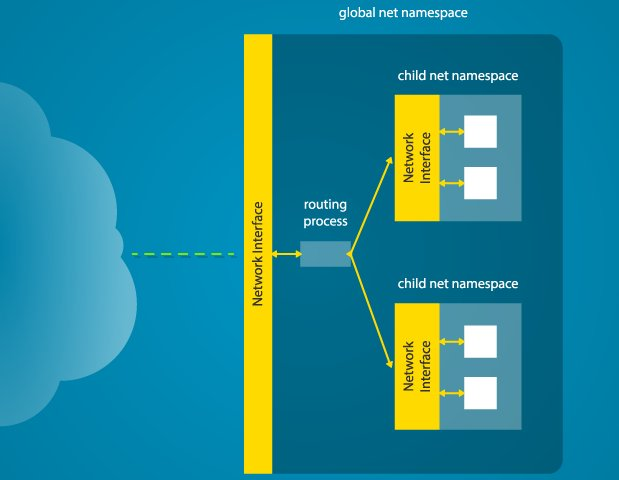
\includegraphics[scale=0.46]{net_ns.jpg}
    \end{figure}
\end{frame}

\begin{frame}[label={net_ns_features}]
\frametitle{Особенности NET NS}
\begin{itemize}
    \item Каждое сетевое устройство может принадлежать только одному сетевому неймспейсу,
    \item Каждый сокет может принадлежать только одному сетевому неймспейсу,
    \item Физические устройства принадлежат только корневому неймспейсу
    \item Для маршрутизации между неймспейсами используется механизм \alert{виртуальных сетевых устройств (veth)}
    \item В отличие от других неймспейсов, сетевые неймспейсы требуют явного освобождения и могут "переживать" использующие их процессы.
\end{itemize}
\end{frame}

\begin{frame}[fragile, label={net_ns_create}]
\frametitle{Создание неймспейсов}
\begin{block}{}
\begin{lstlisting}[language=bash, basicstyle={\fontsize{8}{8}\ttfamily}]
# ip netns add netns1
\end{lstlisting}
    Эта команда создает новый сетевой неймспейс \alert{netns1}. Помимо этого также создается маунт соответствующий неймспейсу в директории \texttt{/var/run/netns}. 
    
    Команда \texttt{ip netns exec} позволяет запускать команды внутри сетевых неймспейсов:
\begin{lstlisting}[language=bash, basicstyle={\fontsize{8}{8}\ttfamily}]
# ip netns exec netns1 ip link list
1: lo: <LOOPBACK> mtu 65536 qdisc noop state DOWN mode DEFAULT 
    link/loopback 00:00:00:00:00:00 brd 00:00:00:00:00:00
# ip netns exec netns1 ping 127.0.0.1
connect: Network is unreachable
# ip netns exec netns1 ip link set dev lo up
# ip netns exec netns1 ping 127.0.0.1
PING 127.0.0.1 (127.0.0.1) 56(84) bytes of data.
64 bytes from 127.0.0.1: icmp_seq=1 ttl=64 time=0.051 ms
\end{lstlisting}
\end{block}

\end{frame}

\begin{frame}[fragile, label={net_ns_delete}]
\frametitle{Освобождение неймспейсов}
\begin{block}{}
\begin{lstlisting}[language=bash, basicstyle={\fontsize{8}{8}\ttfamily}]
# ip netns del netns1
\end{lstlisting}
\begin{itemize}
    \item Отмонтирует \texttt{/var/run/netns/netns1}
    \item Неймспейс не будет освобожден, если он используется хотя бы одним процессом
    \item "Мигрируемые"{} устройства будут перемещены в сетевой неймспейс по умолчанию
    \item "Неперемещаемые"{} устройства (имеющие флаг \texttt{NETIF\_F\_NETNS\_LOCAL} в свойствах) будут уничтожены
    \item Примеры неперемещаемых устройств: loopback, ppp, bridge.
\end{itemize}
\end{block}
\end{frame}

\begin{frame}[fragile, label={ns_net_example}]
\frametitle{Пример}
\begin{block}{}
\begin{lstlisting}[language=bash, basicstyle={\fontsize{6}{6}\ttfamily}]
# modprobe dummy 
# ip addr add 192.168.100.199/24 brd + dev dummy0 
# ip link set dev dummy0 up 
# ifconfig | grep dummy
dummy0  Link encap:Ethernet  HWaddr fa:62:00:cd:d0:c2
# ip link set dummy0 netns netns1 
# ifconfig | grep dummy
# ip netns exec netns1 bash
# ifconfig
dummy0    Link encap:Ethernet  HWaddr fa:62:00:cd:d0:c2  
          inet addr:192.168.100.199  Bcast:192.168.100.255  Mask:255.255.255.0
          ...
# mkdir -p /etc/netns/netns1
# echo '192.168.100.199 dummy.com' > /etc/netns/netns1/hosts
# ping dummy.com
PING dummy.com (192.168.100.199) 56(84) bytes of data.
64 bytes from dummy.com (192.168.100.199): icmp_seq=1 ttl=64 time=0.046 ms
64 bytes from dummy.com (192.168.100.199): icmp_seq=2 ttl=64 time=0.042 ms
\end{lstlisting}
\end{block}
\end{frame}

\begin{frame}[fragile, label={ns_net_veth}]
\frametitle{Виртуальный сетевой интерфейс}
\begin{block}{}
     Взаимодействовать между сетевыми неймспейсами позволяет механизм \alert{виртуальных сетевых интерфейсов (veth)}. Виртуальный сетевой интерфейс напоминает pipe: это пара сетевых интерфейсов связанных друг с другом и находящихся в разных неймспейсах. 

    Создать veth можно следующей командой:
    \begin{lstlisting}[language=bash, basicstyle={\fontsize{8}{8}\ttfamily}]
# ip link add name veth0 type veth peer name veth1 netns <pid>
\end{lstlisting}
    где \texttt{veth0} и \texttt{veth1} \textemdash{} имена сетевых интерфейсов, а \texttt{<pid>} \textemdash{} индентификатор процесса в дочернем сетевом немспейсе.
\end{block}
\end{frame}

\begin{frame}[fragile, label={ns_net_under_hood}]
\frametitle{Под капотом}
    \begin{block}{}
    В ядре сетевой неймспейс представлен структурой \texttt{struct net} объявленной в \texttt{include/net/net\_namespace.h}. В структуре \texttt{struct net\_device} имеется указатель на неймспейс к которому данное сетевое устройство принадлежит.
\begin{lstlisting}[title=\href{http://lxr.free-electrons.com/source/include/linux/netdevice.h}{netdevice.h}]
struct net_device {
    ...
    net* nd_net;
    ...
}
\end{lstlisting}
    С помощью функций \texttt{struct net* dev\_net(const struct net\_device *dev)} и \texttt{void dev\_net\_set(struct net\_device *dev, struct net *net)} можно получить доступ к немспейсу данного сетевого устройства.
\end{block}
\end{frame}


\begin{frame}[fragile]
\frametitle{Под капотом}
    В структуре \texttt{struct sock} также имеется поле \texttt{struct net* sk\_net} а также функции \texttt{sock\_net} и \texttt{sock\_net\_set} для доступа к неймспейсу сокета соответственно.

    Все имеющиеся неймспейсы связаны в список \texttt{extern struct list\_head net\_namespace\_list;}, а макрос \texttt{for\_each\_net()} позволяет проходить в цикле по ним.

    Сетевой неймспейс по умолчанию представлен структурой \texttt{extern struct net init\_net;} включающий в себя loopback и все физические сетевые устройства. 

\end{frame}

\begin{frame}[fragile]
\frametitle{Под капотом}
\begin{block}{}
    \begin{lstlisting}[title=\href{https://github.com/shemminger/iproute2/blob/master/ip/ipnetns.c}{ipnetns.c}, language=c, basicstyle={\fontsize{6}{6}\ttfamily}]
    /* Create the base netns directory if it doesn't exist */
	mkdir(NETNS_RUN_DIR, S_IRWXU|S_IRGRP|S_IXGRP|S_IROTH|S_IXOTH);
	/* Create the filesystem state */
	fd = open(netns_path, O_RDONLY|O_CREAT|O_EXCL, 0);
	if (fd < 0) {
		...	
    }
	close(fd);
	if (unshare(CLONE_NEWNET) < 0) {
		...	
    }

	/* Bind the netns last so I can watch for it */
	if (mount("/proc/self/ns/net", netns_path, "none", MS_BIND, NULL) < 0) {
		...
    }
	return 0;
\end{lstlisting}
\end{block}
\end{frame}

\begin{frame}[fragile, label={}]
\frametitle{Под капотом}
\begin{block}{}
    \begin{lstlisting}[language=c, basicstyle={\fontsize{6}{6}\ttfamily}]
static void __net_exit default_device_exit(struct net *net)
{
        struct net_device *dev, *aux;
        /*
         * Push all migratable network devices back to the
         * initial network namespace
         */
        rtnl_lock();
        for_each_netdev_safe(net, dev, aux) {
                int err;
                char fb_name[IFNAMSIZ];

                /* Ignore unmoveable devices (i.e. loopback) */
                if (dev->features & NETIF_F_NETNS_LOCAL)
                        continue;

                /* Leave virtual devices for the generic cleanup */
                if (dev->rtnl_link_ops)
                        continue;

                /* Push remaining network devices to init_net */
                snprintf(fb_name, IFNAMSIZ, "dev%d", dev->ifindex);
                err = dev_change_net_namespace(dev, &init_net, fb_name);
                if (err) {
                        ...
                }
        }
        rtnl_unlock();
}
\end{lstlisting}
\end{block}
\end{frame}


\begin{frame}
\frametitle{Материалы}
    \begin{itemize}
        \item \href{http://www.haifux.org/lectures/299/netLec7.pdf}{http://www.haifux.org/lectures/299/netLec7.pdf}
        \item \href{https://www.toptal.com/linux/separation-anxiety-isolating-your-system-with-linux-namespaces}{https://www.toptal.com/linux/separation-anxiety-isolating-your-system-with-linux-namespaces}
        \item \href{http://lwn.net/Articles/580893/}{http://lwn.net/Articles/580893/}
    \end{itemize}
\end{frame}

\end{document}
